\begin{figure}[!ht]\centering
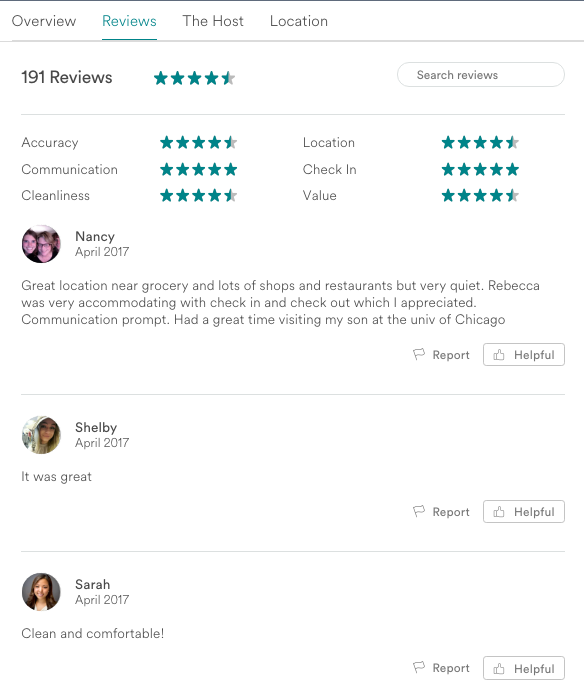
\includegraphics[width=.8\textwidth]{figures/sample3-reviews}
\caption{Sample review information}
	\label{fig:reviewinfo}
\end{figure}
\begin{figure}\centering
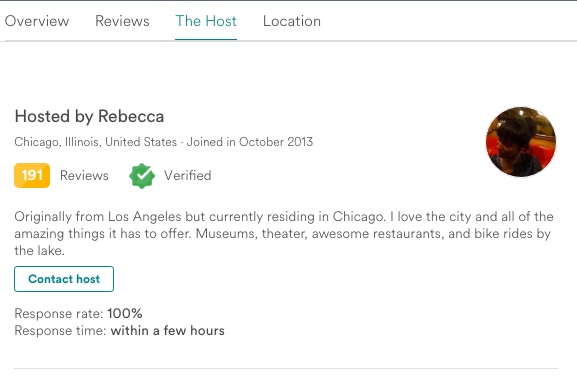
\includegraphics[width=.9\textwidth]{figures/sample4-host}
\caption[Sample host information]{Sample host information available.}
	\label{fig:host}
\end{figure}
\begin{figure}\centering
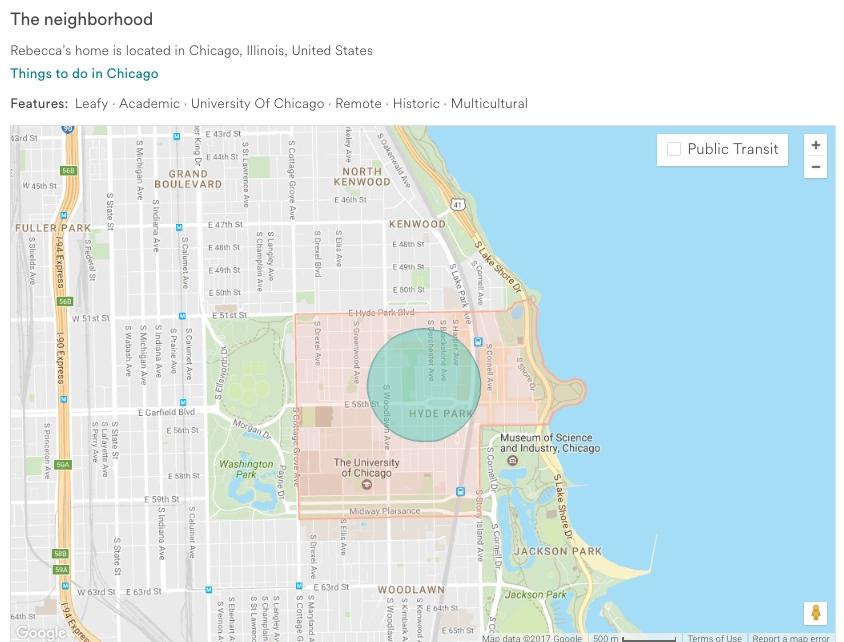
\includegraphics[width=.8\textwidth]{figures/sample5-location}
\caption{Sample location information}
	\label{fig:location}
\end{figure}
\begin{figure}\centering
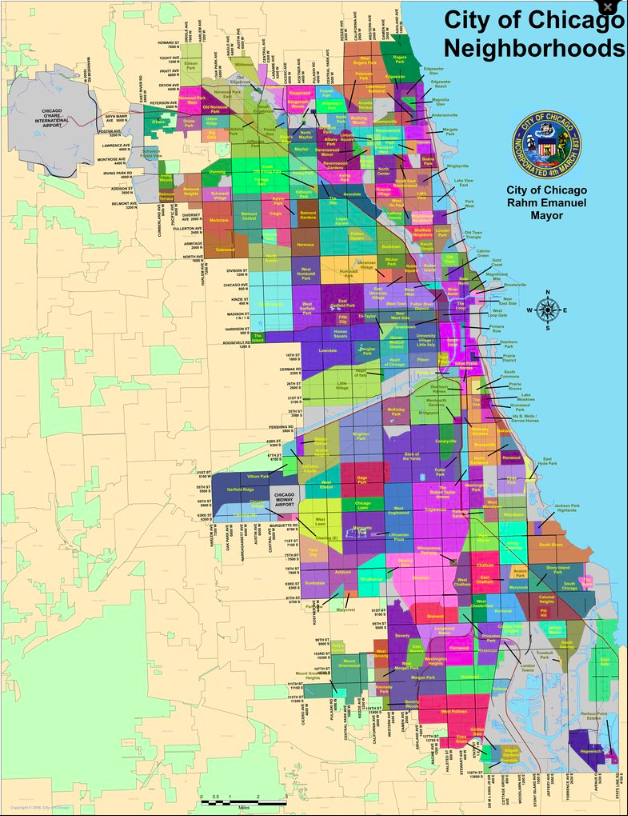
\includegraphics[width=.8\textwidth]{figures/chicago_city_neighborhoods}
\caption[City of Chicago neighborhoods]{City of Chicago neighborhoods, showing level of granularity of neighborhood controls}
	\label{fig:chicago}
\end{figure}


